\documentclass{article}

% Language setting
% Replace `english' with e.g. `spanish' to change the document language
\usepackage[polish]{babel}

% Set page size and margins
% Replace `letterpaper' with `a4paper' for UK/EU standard size
\usepackage[a4paper,top=2cm,bottom=2cm,left=3cm,right=3cm,marginparwidth=1.75cm]{geometry}

% Useful packages
\usepackage{amsmath}
\usepackage{graphicx}
\usepackage[pdftex,
            pdfauthor={Michał Czyż, Dawid Głąb},
            pdftitle={PK - Sprawozdanie},
            pdfsubject={Sprawozdanie},
            pdfkeywords={PK4, Projekt, Sprawozdanie},
            pdfproducer={Latex with hyperref},
            pdfcreator={pdflatex},
            colorlinks=true,
            allcolors=blue]{hyperref}

\usepackage[T1]{fontenc}

\usepackage[skip=5pt plus1pt, indent=20pt]{parskip}

\usepackage{listings}

\title{%
  PK4: Platforma NLP \\
  \large Sprawozdanie}

\author{Michał Czyż}

\begin{document}
\maketitle

\section{Wstęp}

Projektem przewidzianym do wykonania w tym semestrze była platforma przetwarzania języka naturalnego \textit{(eng. natural langugage processing)}. W ramach projektu zaimplementowane zostało tłumaczenie tekstu, wykrywanie języka tekstu, anonimizacja danych wrażliwych, oraz badanie sentymentu. 

Przetwarzanie języka naturalnego to dziedzina nauki łącząca językoznawstwo oraz dziedzinę sztucznej inteligencji. Zajmuje się ona analizą i przetwarzaniem języka ludzkiego przez komputer. Po stworzeniu i wyszkoleniu modelu językowego, program jest w stanie z dużą dokładnością przewidywać oraz wykryć logiczny ciąg zdań języka. Na tej podstawie może być on dalej analizowany i przetwarzany.

Tłumaczenie maszynowe może być realizowane na wiele różnych sposobów. Skupiono się na dwóch rozwiązaniach jakimi są statystyczne tłumaczenie maszynowe oraz duże modele językowe opartych na transformerach. Do tłumaczenia statystycznego wykorzystano pierwszy model opracowany przez IBM w latach 90. Skupia się on w głównej mierze na tłumaczeniu leksykalnym, zatem nie będzie bardzo dokładny przy wychwytwaniu dokładnego kontekstu, ale jest w stanie osiągnąć dostateczne rezulataty. Dodatkowym atutem tego modelu jest jego wysoka wydajność. Model oparty jest o prawdopodobieństwo warunkowe.

\section{Analiza tematu}

Platforma NLP składa się z trzech usług:

\begin{itemize}
  \item Core - główny program napisany w języku C++. Jest to główny program skupiający się na komunikacji z warstwą API oraz na przetwarzaniu danych.
  \item Middleware - serwer API, napisany w Pythonie. Łączączy komunikację pomiędzy użytkownikiem, a programem głównym. Middleware udostępnia warstwę programistyczną, którą wykorzystuje frontend.
  \item Frontend - strona internetowa napisana przy pomocy Next.JS oraz Reacta. Korzysta z API i udostępnia wartswę graficzną użytkownikowi końcowemu.
\end{itemize}

\noindent Język C++ wybrano przede wszystkim ze względu na wydajność oraz dostępność wielu elementów programowania obiektowego. Język Python został wybrany, ponieważ ma bardzo rozbudowane biblioteki do nauczania maszynowego oraz posiada bardzo łatwe i wygodną bibliotekę - \textit{Flask}.

Jednym z głównych założeń projektu jest bycie modularnym i łatwym w rozbudowie. W szczegółności, iż projekt jest złożony i wymaga wykorzystania wielu języków i bibliotek. Główna struktura programu w C++ wygląda następująco:

\begin{itemize}
  \item Communication - zajmuje się komunikacją pomiędzy pythonem i programem.
  \item Engine - zbiór wielu klas obsługujących działanie programu i przetwarzających dane.
  \item Translate - zbiór klas odpowiedzialnych za obsługę tłumaczenia.
  \item Sentiment - zbiór klas odpowiedzialnych za obsługę analizy sentymentu.
  \item AsyncLogger - klasa odpowiedzialna za prawidłowe logowanie stanu programu.
\end{itemize}

Wykorzystanie biblioteki podczas tworzenia głównego programu w C++ to zeromq, cppzmq oraz boost. ZeroMQ jest wykorzystywany do komunikacji pomiędzy programem a interfejsem sieciowym. Biblioteka cppzmq udostępnia wygodny sposób do inicializacji i zarządzania komunikacją. Biblioteka Boost była używana przy łączeniu C++ z Pythonem oraz do komunikacji.

\begin{figure}[h!]
\centering
  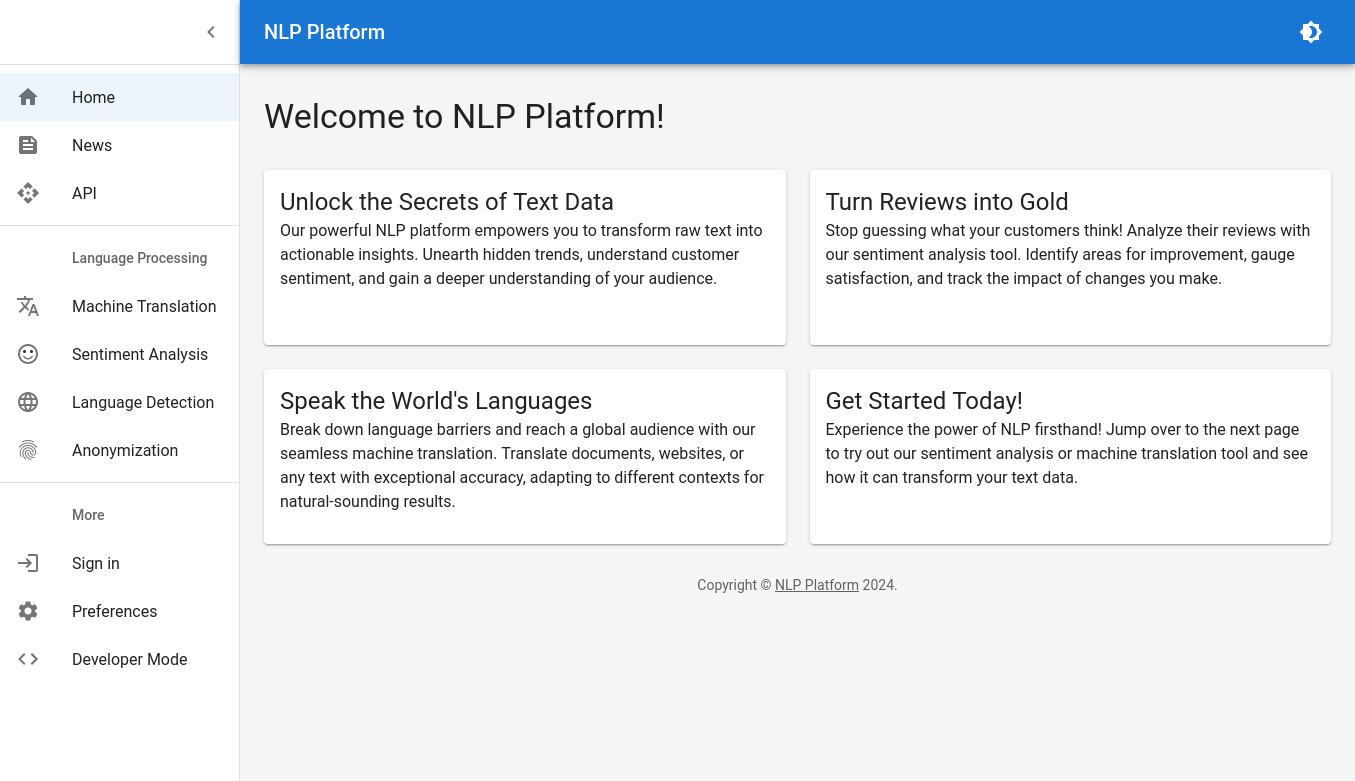
\includegraphics[width=1\linewidth]{img/nlp-dashboard.png}
  \caption{\label{fig:nlp dashboard}Wygląd srony głównej}
\end{figure}

\section{Specyfikacja zewnętrzna}

Program posiada warstwę API oraz graficzną co pozwala na interakcję z platformą w wygodny sposób dla użytkownika końcowego jak i także dla programisty, który chciałby wykorzystać funkcjonalność platformy NLP w swoim programie. Serwer API posiada podstawową autoryzację poprzez token API.

\begin{figure}[h!]
\centering
  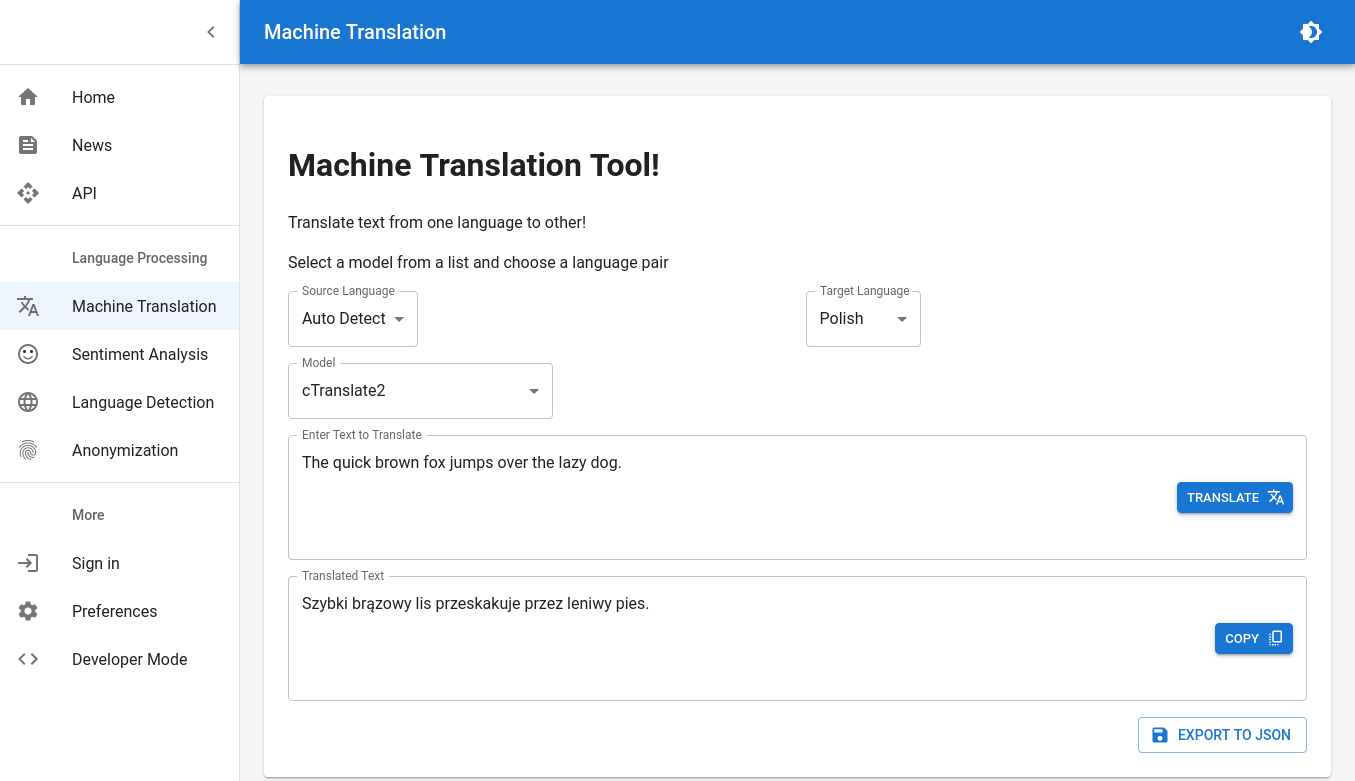
\includegraphics[width=1\linewidth]{img/nlp-translate.png}
  \caption{\label{fig:nlp translation}Interfejs tłumaczenia maszynowego}
\end{figure}

\subsection{Instrukcja dla użytkownika}

Jeżeli usługa jest uruchomiona na komputerze lub port interfejsu webowego jest udostępniony do internetu wystarczy, że użytkownik ma dostęp do internetu oraz posiada zainstalowaną przeglądarkę internetową. Po odwiedzeniu odpowiedniego adresu ukaże się strona internetowa po której może nawigować i wybierać interesujące go funkcje.  

\subsection{Przykłady działania}

Przykłady działania aplikacji zostały przedstawione na rysunkach widocznych w dokumencie. Jest możlwie swobodne nawigowanie po interfejsie webowym, wybranie modelu i pary językowej, która nas interesuje oraz odczytanie i pobranie wyniku w postaci pliku JSON. 

\begin{figure}[h!]
\centering
  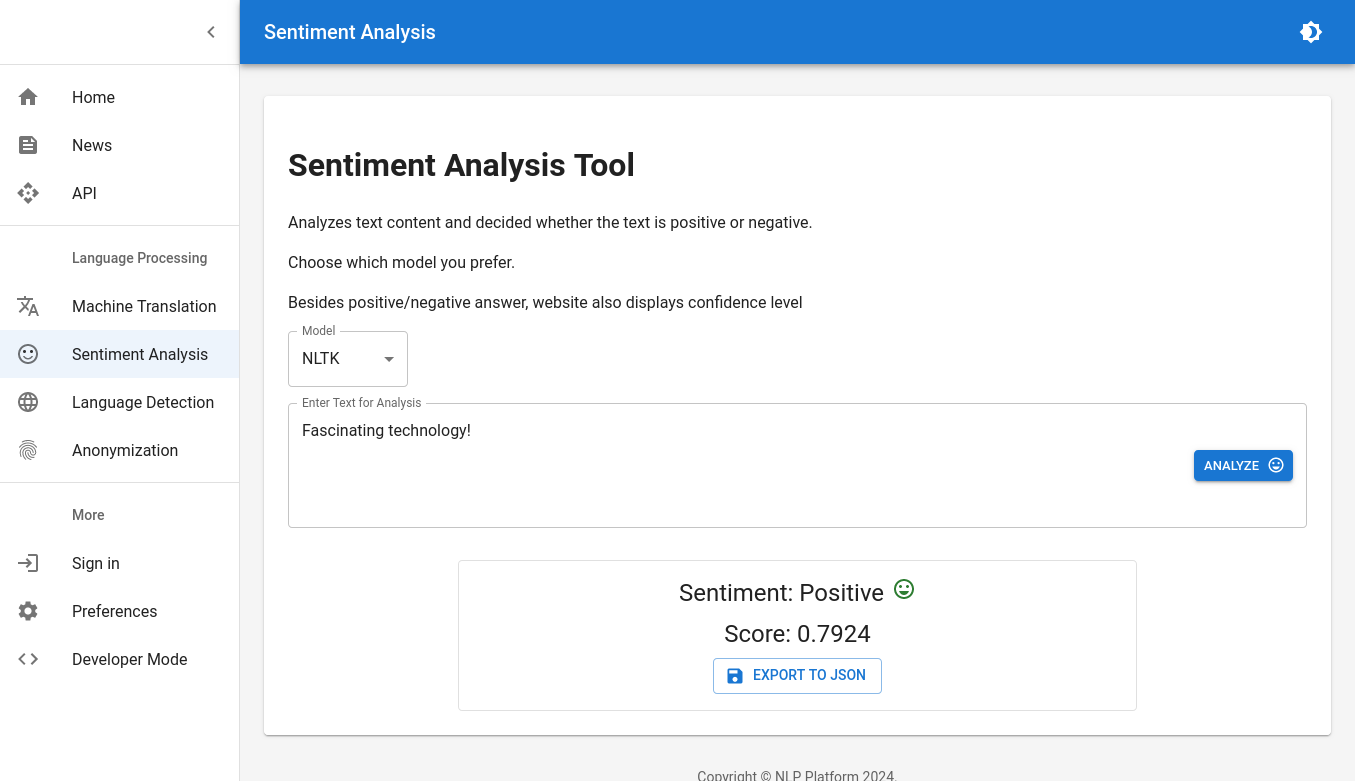
\includegraphics[width=1\linewidth]{img/nlp-sentiment.png}
  \caption{\label{fig:nlp sentiment}Interfejs analizy sentymentu}
\end{figure}

Interfejs Programowania Aplikacji wygląda następująco. Należy wysłać zapytanie na następującą scieżkę na serwerze:

\begin{lstlisting}
GET http://localhost:8080/api/ping

POST http://localhost:8080/api/translate
POST http://localhost:8080/api/sentiment
POST http://localhost:8080/api/detect
POST http://localhost:8080/api/anonymize

POST http://localhost:8080/api/auth
POST http://localhost:8080/api/signin
\end{lstlisting}

\noindent Struktura dla przykładowego tłumaczenie przy wykorzystaniu cTranslate2 wygląda następująco:

\begin{lstlisting}
{
  "srcLanguage": "en",
  "dstLanguage": "pl",
  "mode": "ct2",
  "data": "Natural Language Processing"
}
\end{lstlisting}

\section{Specyfikacja wewnętrzna}

\begin{figure}[h!]
\centering
  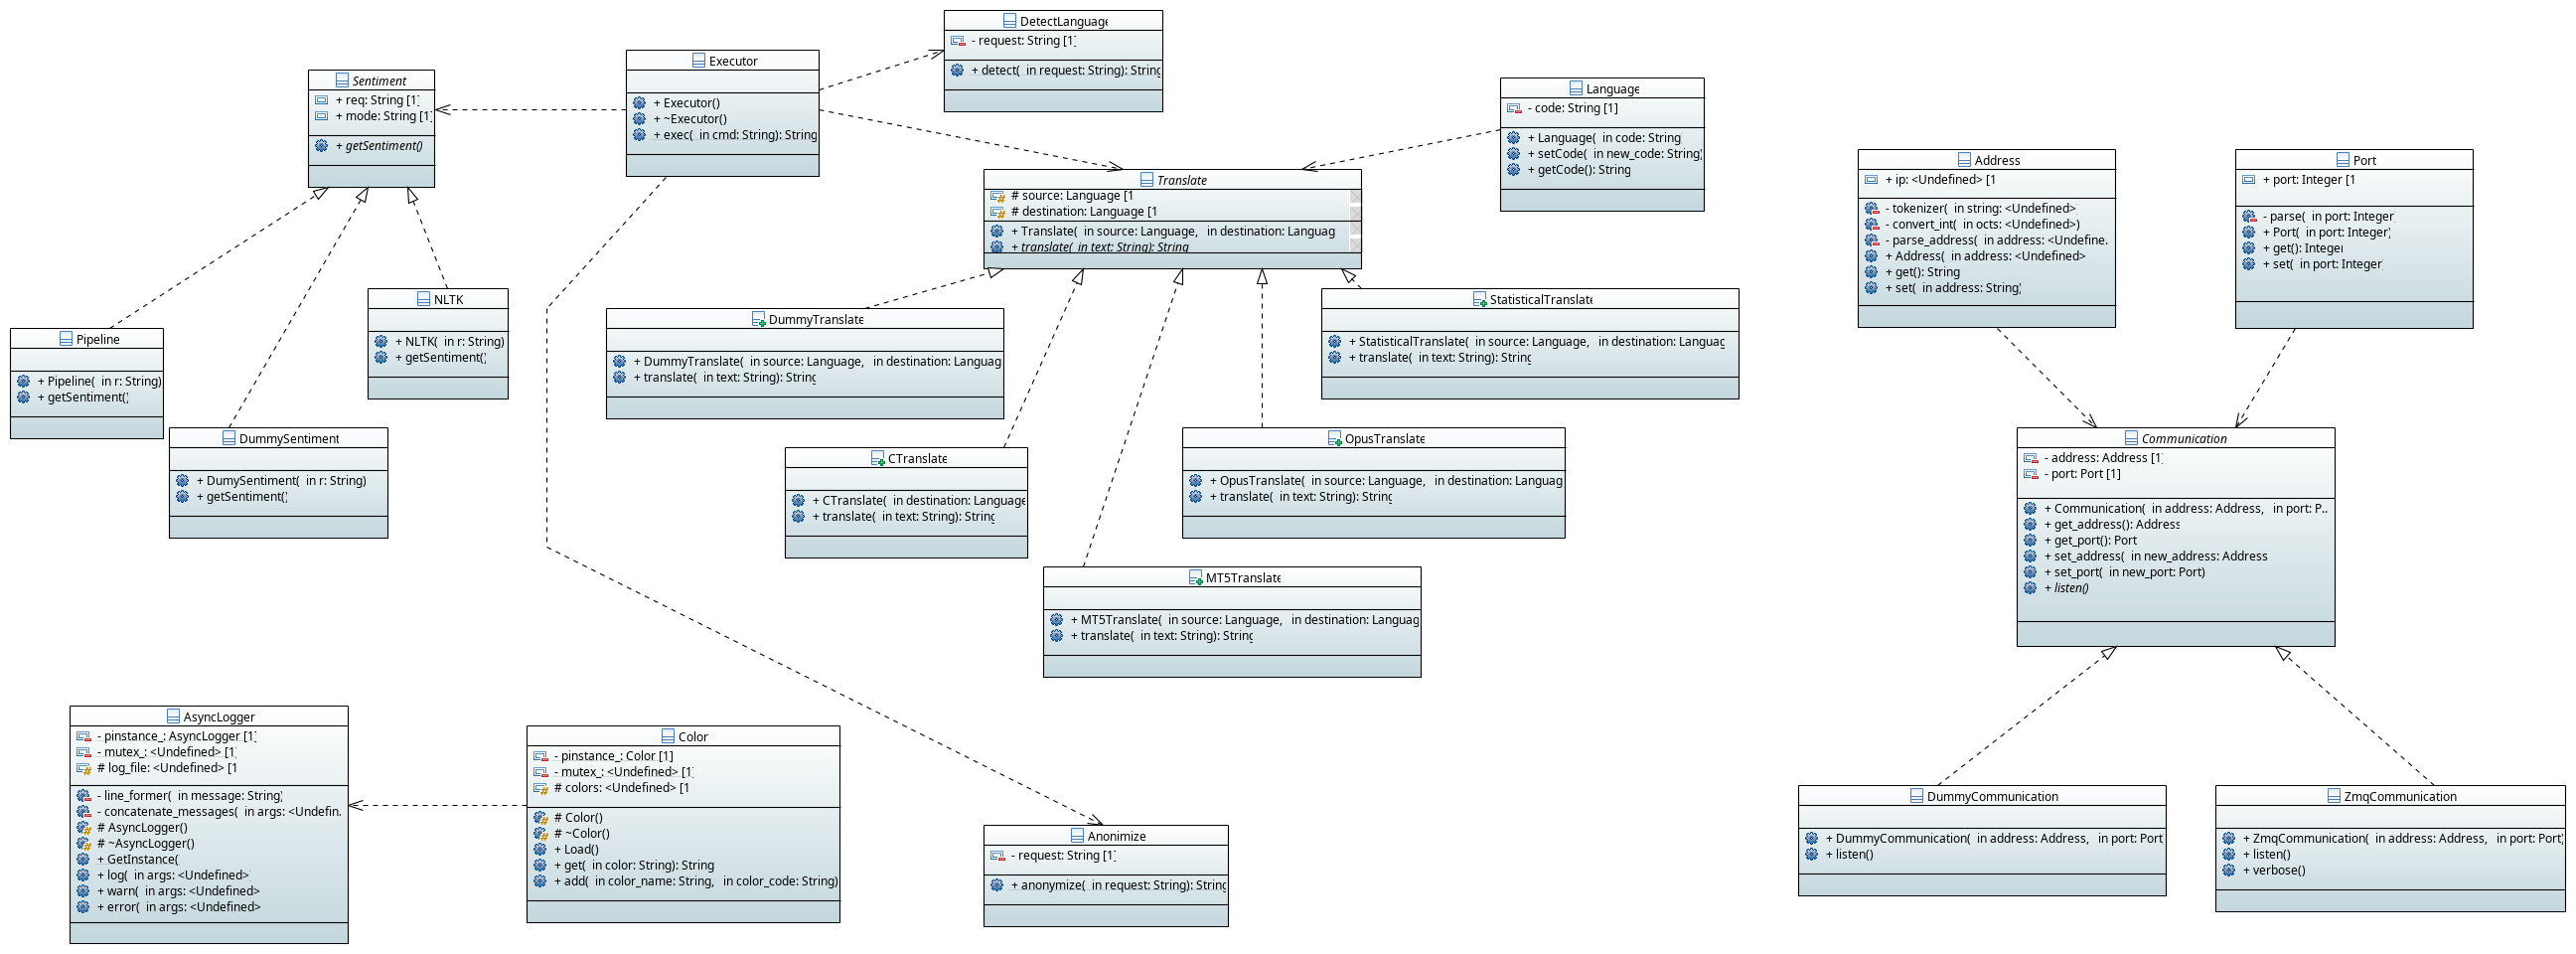
\includegraphics[width=1\linewidth]{img/Class_Diagram.PNG}
  \caption{\label{fig:class diagram}Diagram Klas}
\end{figure}

Diagram klas został przedstawiony na Rysunku 4. Główne klasy to Translate, Communication oraz Sentiment, które odpowiadają za główną funkcjonalność programu.
Reszta klas to m.in. AsyncLogger - odopowiedzialny za logowanie danych do pliku i do konsoli. Klasy DetectLanguage oraz Anonymize, które są odpowiedzialne za detekcję i anonimizację danych. 

Zostały także utworzone klasy Dummy, które symulują tylko swe działanie. Jest zwracana tylko stała odpowiedź. Jest to przydatne przy debuggowaniu i implmentacji konkretnych części aplikacji. 

Z technik obiektowych wykorzystano m.in. polimorfizm. Kluczowe było to, aby program był bardzo modularny i aby była możliwość modyfikacji każdej funkcjonalności programu. Drugim ważnym czynnikiem była także skalowalność programu. 

Wykorzystano wzorzec projektowy Singleton, który zapewnia tylko jedną instancję danej klasy. Klasa AsyncLogger jest zaawansowaną klasą zajmującą się logowaniem statusu i działania programu. Został napisany jako Singleton aby zapewnić bezpieczeństwo zapisu do pliku i do standardowego wyjścia przy działaniu wielu wątków równolegle.

\noindent Wykorzystane elementy z laboratorium to: 
\begin{itemize}
  \item Wyrażenia regularne do weryfikacji przepływu danych oraz poprawności przekazywanych danych.
  \item Ranges do łatwego przechodzenia przez pętle.
  \item Asynchroniczność do poprawnego zapisu do pliku i konsoli.
  \item Wielowątkowość do prawidłowej obsługi workerów i brokera do komunikacji z API.
  \item Koncepty do weryfikacji danych i zmiennych jakie są przekazywane do funkcji i template'ów.
\end{itemize}

Niewykorzystane zostały moduły z tego powodu iż program wykorzystuje kompilator G++, który nie wspiera ich dobrze. Drugim niewykorzystanem elementem laboratorium była biblioteka filesystem, ponieważ program nie posiada żadnej zaawansowej obsługi systemu plików.

Działanie programu wygląda następująco. Po odebraniu zapytania, serwer API sprawdza czy request jest poprawny. Jeżeli request jest poprawny, jest on parsowany i przekazywany do C++. Kiedy odbierze to C++, request jest dokładnie analizowany i wybierane są konkretne parametry. Po analizie wyborów, następuje przekazanie do konkretnej metody z konkretnymi parametrami. Metoda w konkretnej klasie wywołuje instancję Executora, który poprawnie wysyła i odbiera wynik z częsci Pythonowej. Nastepnie wynik jest zwracany do API. API, pakuje wynik do JSONa i zwraca go użytkownikowi końcowemu.

\noindent Wykorzystane modele i datasety do trenowania:
\begin{itemize}
  \item \href{https://huggingface.co/santhosh/madlad400-3b-ct2}{Madlad400 3b CT2}
  \item \href{https://github.com/Mimino666/langdetect}{Langdetect Library}
  \item \href{https://huggingface.co/google/mt5-base}{Google MT5 Base}
  \item \href{https://huggingface.co/jproboszcz/opus-mt-en-pl}{Opus MT}
  \item \href{https://www.nltk.org/_modules/nltk/translate/ibm1.html}{NLTK IBM Model 1}
  \item \href{https://microsoft.github.io/presidio/analyzer/}{Presidio Analyzer}
  \item \href{https://www.kaggle.com/datasets/martininf1n1ty/ankiweb-polish-english}{AnkiWeb Polish-English Vocabulary}
  \item \href{https://www.kaggle.com/datasets/ahmadiub/languages-dataset}{European Parliament Languages Dataset}
\end{itemize} 

\section{Testowanie}

Program był testowany w kilku etapach. Na początku testowano interfejs webowy aby sprawdzić czy wszystkie możliwości i kombinacje ustawień modeli są prawidłowe. Sprawdzana była także komunikacja warstwy webowej z API oraz czy wszystkie requesty są poprawnie obsługiwane lub odrzucane.

Póżniej sprawdzano poprawność działania warstwy API z warstwą C++. Komunikacja ta była kluczowa do poprawnego działania programu. Sprawdzono także czy wszystkie przekazywane dane są przekazywane prawidłowo, czy nie można poprzez wysłanie błędnych danych dokonać \textit{remote code execution}.

Ostatecznie sprawdzano warstwę C++, pod kątem bezpieczeństwa wykonywania modeli. A także testowano czy wszstkie klasy zachowują się zgodnie z założeniem.

\section{Uruchamianie}

Zalecana kolejność uruchamiania usług to warstwa webowa, następnie API i na końcu program w C++.

\subsection{Uruchomienie serwera WWW}

Wymagane pakiety: \texttt{nodejs}, \texttt{npm}

\noindent Aby uruchomić usługę należy wykonać następujące kroki:

\begin{lstlisting}
$ cd web
$ npm install
$ npm run build
$ npm run start
\end{lstlisting}

\noindent Aplikacja uruchomi się na porcie \textit{3000}.

\noindent W przypadku chęci debuggowania aplikacji lub wprowadzania zmian w kodzie można uruchomić serwer deweloperski:

\begin{lstlisting}
$ npm run dev
\end{lstlisting}

\subsection{Uruchomienie serwera API}

Wymagane pakiety: \texttt{python}, \texttt{python-pip}

\begin{lstlisting}
$ cd api
\end{lstlisting}

\noindent Przed uruchomieniem serwera należy aktywować wirtualne środowisko.

\begin{lstlisting}
$ source activate.sh
\end{lstlisting}

\noindent Potem można wywołać serwer API.

\begin{lstlisting}
$ python main.py
\end{lstlisting}

\noindent Aby opuścić wirtualne środowisko, można wykonać polecenie:

\begin{lstlisting}
$ deactivate
\end{lstlisting}

\subsection{Uruchomienie Core Platform}

Wymagane pakiety: \texttt{base-devel}, \texttt{boost}, \texttt{cmake}, \texttt{python}, \texttt{python-pip}, \texttt{mold}, \texttt{zeromq}, \texttt{cppzmq}

\noindent Na początku należy aktywować wirtualne środowisko, aby móc wykorzystywać modele.

\begin{lstlisting}
$ cd nlp/models
\end{lstlisting}

\noindent Umożliwia to skrypt activate.sh.

\begin{lstlisting}
$ source activate.sh
$ cd ..
\end{lstlisting}

\noindent Ostatecznie wystarczy skompilować i uruchomić program wykonując:

\begin{lstlisting}
$ make
\end{lstlisting}

\noindent Jeżeli nie chcemy ponownie kompilować programu, można wykorzystać:

\begin{lstlisting}
$ make run
\end{lstlisting}

\noindent Aby opuścić wirtualne środowisko, można wykonać polecenie:

\begin{lstlisting}
$ deactivate
\end{lstlisting}

\subsection{Parametry programu}

W C++ można także przekazać parametr --verbose, który włącza dodatkowe logowanie do konsoli informacji o działaniu ZeroMQ i dokładnego przebiegu pakietów.

\section{Uwagi i wnioski}

Podsumowując, platforma NLP okazała się fascynującym i bardzo rozwojowym projektem. Poznałem jak działają modele językowe, jak tworzyć i trenować własne. Nauczyłem się także jak łączyć warstwę sieciową z programami niższego poziomu, jak C++. Mogłem także dobrze rozwinąć swoje umiejętności programowania obiektowego oraz poznać i lepiej zgłębić zagadnienia poznane w ramach laboratorium.

\end{document}
